\documentclass[10pt]{article}
\usepackage[top=1cm,bottom=1cm,left=1cm,right=1cm]{geometry}
%\usepackage{fontspec}
\usepackage{hyperref}
\usepackage{enumitem}
%\setlist{nolistsep}
\usepackage{changepage}
\usepackage[table]{xcolor}
\usepackage{graphicx}
\hypersetup{
	colorlinks=true,      
	urlcolor=magenta,
}
\newcommand{\main}{\par\noindent\hspace*{0pt}\ignorespaces}
\newcommand{\sub}{\par\noindent\hspace*{100pt}\ignorespaces}
\begin{document}
	\pagenumbering{gobble}
	\large
	{\Huge\noindent\hspace*{200pt}\textbf{Ayush Gaurav}}
	\vspace{.5cm}
	\hrule
	\begin{minipage}{0.4\textwidth}
		\begin{flushleft}
			\textbf{Address:}17 Meena Enclave,\\
			Near Shankar Ashram\\
			Jwalapur, Haridwar\\
			Uttrakhand\\
			249407 \\
			\textbf{Contact:} +91-9565379408\\
			\textbf{email-id:} \href{mailto:ayush23gaurav@gmail.com}{ayush23gaurav@gmail.com}
		\end{flushleft}
	\end{minipage}
	\hfill
	\begin{minipage}{0.4\textwidth}
		\begin{flushright}
			\raisebox{0cm}{\href{run:./resumePic.jpg}{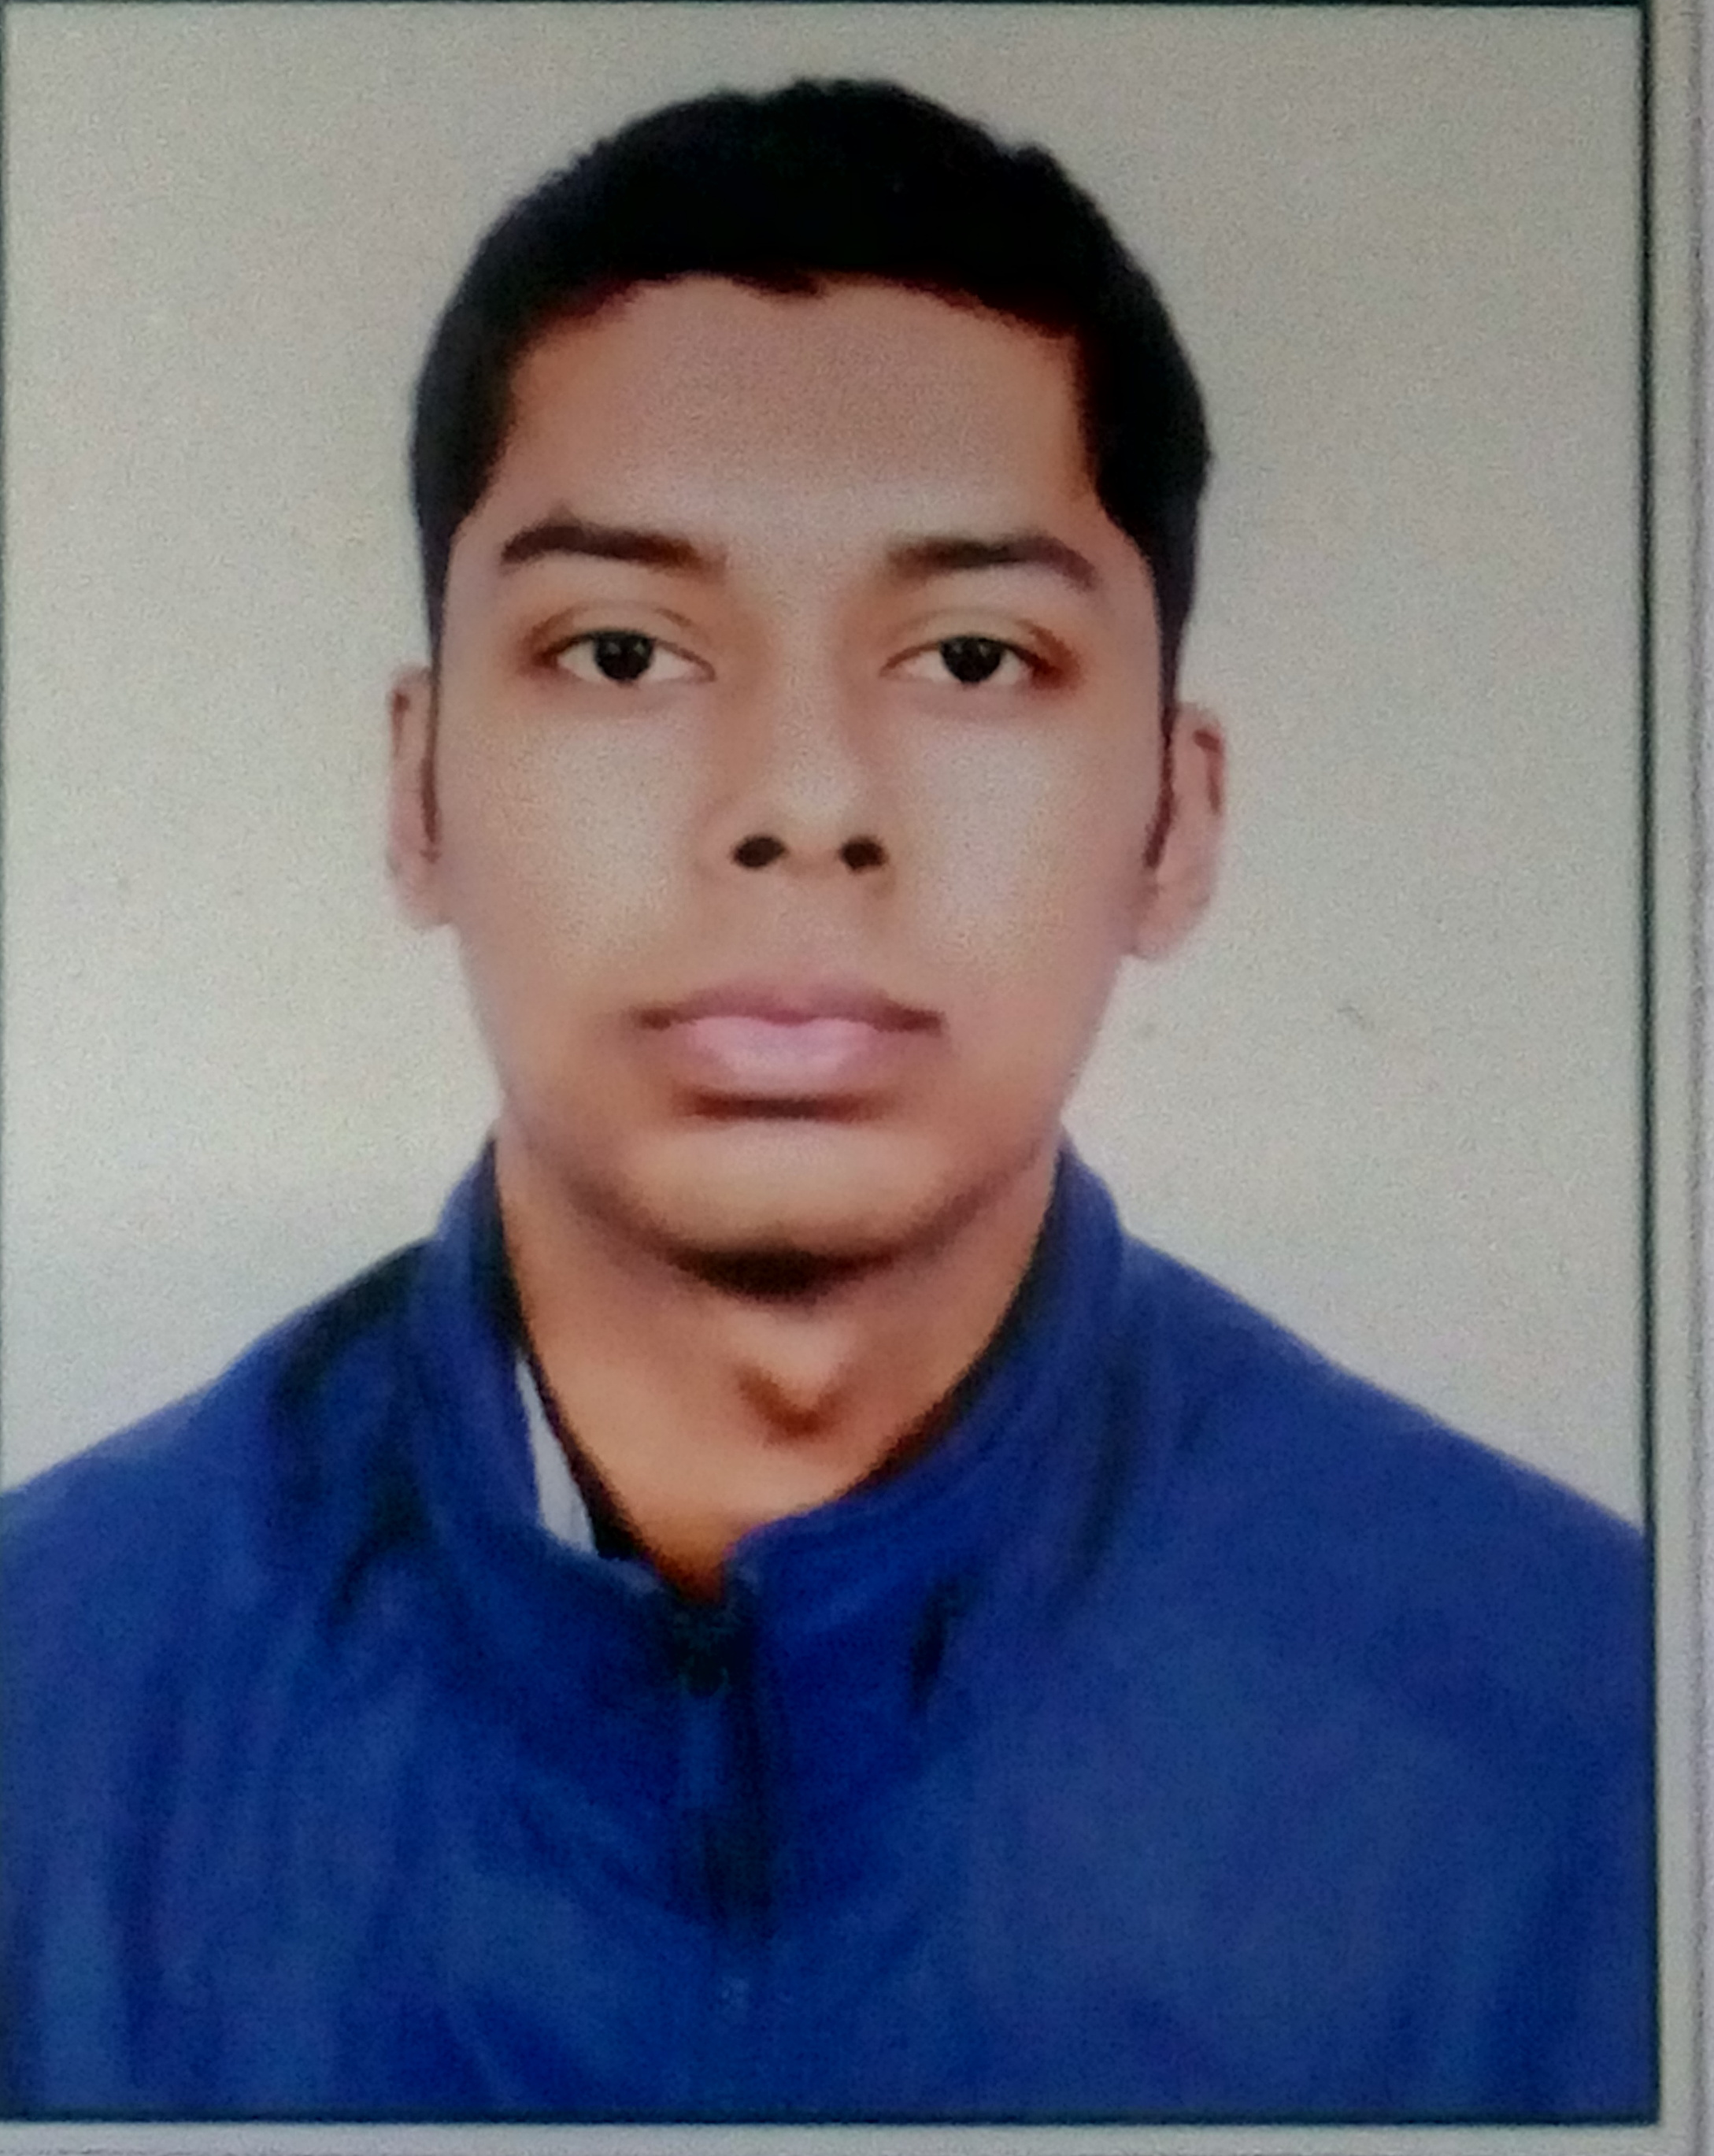
\includegraphics[width=3.5cm]{resumePic.jpg}}}
		\end{flushright}
	\end{minipage}
	\hrule
	\vspace{0.5cm}
		\par{\Large\noindent\textbf{CAREER OBJECTIVE:}} 
	TO WORK HARD IN AN ORGANIZATION OR INDUSTRY WHICH ALLOWS OPPORTUNITY TO INNOVATE, GROW AND DEVELOP
	\main{\textbf{EDUCATION:}}
	\begin{center}
		\begin{tabular}{ |c|c|c|c|c|} 
			\hline
			Degree & College/School & University/Board & Passing Year & Pass Percentage/Grade \\
			\hline 
			B.Tech(ECE) & MNNIT Allahabad & MNNIT Allahabad & 2018 & 8.36/10\\
			\hline
			10th & STCS Srinagar Uttrakhand & ICSE & 2012 & 91\%\\
			\hline
			12th & DPS Noida & CBSE & 2014 & 92.4\%\\
			\hline
		\end{tabular}
	\end{center}

\main{\Large\textbf{PROJECTS:}}
\begin{enumerate}
	\item \textbf{Model A Terrain(eYRC Sponsored by MHRD India)}
	\begin{itemize}
		\item Traversal of 5x5 cells.
		\item Finds all the special paths(Curve,Slope,Bump,And Tunnel),obstacles and different colored objects.
		\item Map it onto blender animation software in real time.
		\item Link:\href{https://youtu.be/Ugt36jvnVoE}{eYRC MT50 Demonstration for original configuration}
	\end{itemize}
	\item\textbf{Room Automation}								
	\begin{itemize}		     
		\item Automatic Control of
		\begin{itemize}
			\item Main door entrance (IR sensor)
			\item Fan speed according to the temperature( lm35 sensor)
			\item Intensity level of bulb according to intensity of the room
			\item Curtains according to intensity of outside
		\end{itemize}
		\item Password protected door lock of the room
		\item Triacs and optocoupler is used for voltage control by phase angle variation method
	\end{itemize}
	\item \textbf{DCT of 8x8 image using Spartan 3A kit}						
	\begin{itemize}
		\item IEEE 754 floating point representation
		\item floating point arithmetic unit 
		\item Vga interfacing and keyboard interfacing
	\end{itemize}
	
	\item \textbf{16X2 Lcd Interfacing And UART Implementation On FPGA Kit}
	\begin{itemize}
		\item 	Hyper Terminal was used to communicate with Spartan 3A kit.
		\item 	Transmitted character was also displayed on a 16x2 alphanumeric lcd. 
		\item	Finite State Machine was created using Verilog HDL.	
	\end{itemize}
\end{enumerate}
\newpage
	\main{\Large\textbf{TRAINING \& INTERNSHIP}}\begin{itemize}
	\item \begin{minipage}{0.6\textwidth}
		\begin{flushleft}
			iERS(i3indya for Embedded Systems And Robotics)
		\end{flushleft} 
	\end{minipage}
	\hfill
	\begin{minipage}{0.2\textwidth}
		\begin{flushright}
			{1 Month}
		\end{flushright}
	\end{minipage}
	Brief introduction and familiarization with Embedded Systems and Robotics and extensive study about ATmega 16.
	
\end{itemize}
	\main{\Large\textbf{AREA OF INTEREST:}}
\begin{itemize}
	\item Digital Electronics
	\item Electronic Devices (BJT, MOSFETS  And Operational Amplifiers )
	\item Circuit Design
	\item FPGA(Using Verilog)
\end{itemize}
	\main{\Large\textbf{TECHNICAL SKILLS:}}
\begin{itemize}
	\item	C/C++
	\item	Embedded C
	\item	Verilog HDL
	\item	Matlab
	\item 	Xilinx ISE
	\item Circuit Designing
\end{itemize}
	\main{\Large\textbf{SOFT SKILLS}}
\begin{enumerate}
	\item Leadership
	\item Dedication.
	\item Teamwork.
	\item Problem Solving
	\item Communication Skills
\end{enumerate}
	\main{\Large\textbf{EXTRA- CURRICULAR AND CO- CURRICULAR ACTIVITIES}}
\begin{itemize}
	\item Playing Table Tennis and Cricket
	\item Reading Quora
\end{itemize}
	\main{\Large\noindent\Large\textbf{PERSONAL DETAILS}}
\sub\textbf{{Father's Name:} Rajiv Kumar}
\sub{\textbf{Mother's Name:} Sushila}
\sub{\textbf{Sex:} Male}
\sub{\textbf{Date of Birth:}March,15 1997}
\sub{\textbf{Nationality:} Indian}
\sub{\textbf{Marital Status:} Single}\\
\main{\Large \textbf{REFERENCE:}} eRTS lab IIT Bombay
\end{document}